\documentclass[../../hardware_design_intro/hardware_design_intro.tex]{subfiles}

\begin{document}
    
The listener tracking model is a combination of face detection and stereo vision 
technique for estimating depth.

\subsubsection{Face detection}

We must classify and sort out the entities from the rest of the objects from the 
surroundings to align the speakers properly.

In our case, these entities are people who are listening to the system. To classify 
them from other objects from surroundings, we implement the Harr cascade face detection 
algorithm to sort and cluster out these entities.

Harr cascade is a cascade classifier that implements a machine learning approach based 
on the Adaboost meta-algorithm.

The rectangular shape of the face is meaningful in initializing the classifier. Further, 
the algorithm focuses on the property that the eyes region is often darker than the face 
and nose region. The second feature proposes that the eyes are darker than the bridge of 
the nose. Similarly, this approach finds the entity's possible relations and features 
and records the features for further prediction. 

Once the face is detected, we can obtain the face's location from the origin (center of 
the image).

\subsubsection{Stereo Vision}

Stereo vision compares the information about a scene from two vantage points and 
examining relative positions of objects in the two panels.

An image can be termed as a grid of pixels within some range of indices. Using face 
detection, we narrowed down the object's position in the grid of pixels (x, y). 

Stereo vision gives two images of the same scene from different positions in the same 
plane. Each image gives the deviation of the image from the origin of that respective 
image.

\begin{figure*}
    \centering
    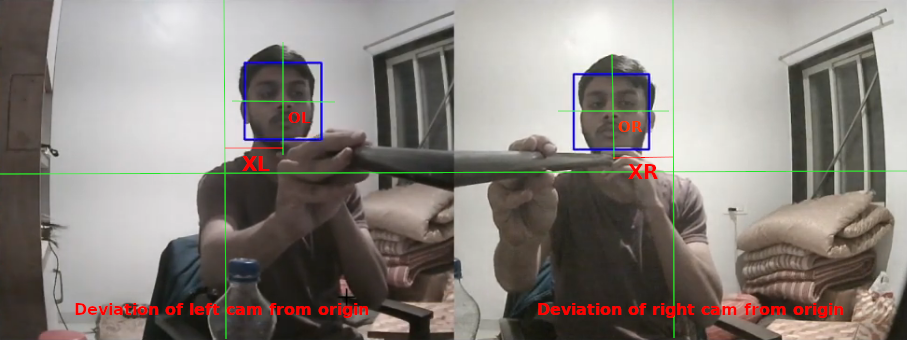
\includegraphics[width=\textwidth]{stereo_vision_pixel_xl_xr.png}
    \caption{Stereo vision showing the deviation from origins of both the cameras}
\end{figure*}

\FloatBarrier

\begin{figure}[ht]
    \centering
    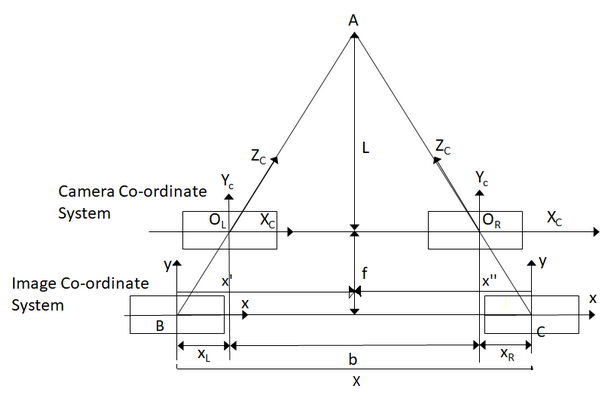
\includegraphics[width=\columnwidth]{stereo_vision_geometry.png}
    \caption{Depth sensing geometrical model}
\end{figure}

\FloatBarrier

Figure 5.1 shows us the geometry behind the stereo vision method for depth sensing.

Here, 

\begin{description}
    \item[]x = Distance between two webcams. 
    \item[]f = Focal length of the webcams.
    \item[]\(X_{L}\) = Deviation of the image from the origin of the left webcam.
    \item[]\(X_{R}\) = Deviation of the image from the origin of the right webcam.  
\end{description}

\begin{figure}[ht]
    \centering
    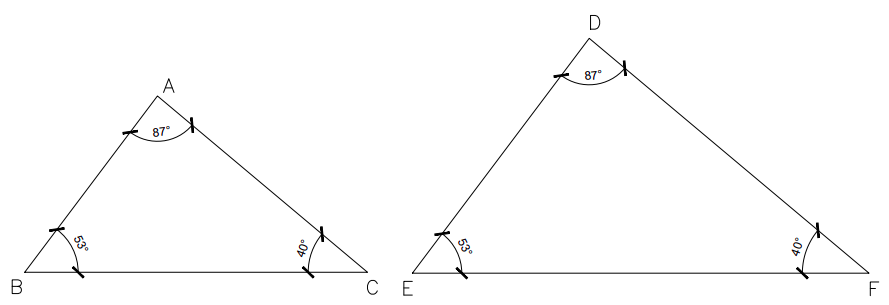
\includegraphics[width=\columnwidth]{aa_criterion.png}
    \caption{AA symmetry criterion}
\end{figure}

Stereo vision depth-sensing works on the principle of angle-angle symmetry (AA symmetry 
criterion) of two triangles. Using the AA symmetry criterion, we can state that if two 
triangle's angles are congruent, then the third angle of both triangles must be the 
same. Hence, the ratio of each parallel side of triangles is equal.

i.e.,

\begin{equation}
    \text{\large$ \frac{AB}{DE} = \frac{BC}{EF} = \frac{AC}{DF} $}
\end{equation}

Hence from figure 5.2, we can prove that,

\begin{equation}
    \text{\large$ \frac{f}{z} = \frac{X_{L}}{X'} $}
\end{equation}

Where, \(z = f + L \),

Similarly,

\begin{equation}
    \text{\large$ \frac{f}{z} = \frac{X_{R}}{X''} $}
\end{equation}

From equation 5.2 and 5.3, we can say that,

\begin{equation}
    \text{\large$ x' = \frac{z \times X_{L}}{f} $}
\end{equation}

\begin{equation}
    \text{\large$ x'' = \frac{z \times X_{R}}{f} $}
\end{equation}

From figure 5.2 we can say that \(x = x' + x'' \),

\begin{align*}
    \therefore{}&\text{\large$ x = \frac{z \times X_{L}}{f} + \frac{z \times X_{R}}{f} $}\\\\
    \therefore{}&\text{\large$ x = \frac{z}{f} \times (X_{L} + X_{R}) $}
\end{align*}

Finally, we get depth (z),

\begin{equation}
    \boxed{\text{\large$ z = \frac{x \times f}{X_{L} + X_{R}} $}}
\end{equation}

\end{document}
